% ----------------------------------------------------------------- %
%             The Speech Signal Processing Toolkit (SPTK)           %
%             developed by SPTK Working Group                       %
%             http://sp-tk.sourceforge.net/                         %
% ----------------------------------------------------------------- %
%                                                                   %
%  Copyright (c) 1984-2007  Tokyo Institute of Technology           %
%                           Interdisciplinary Graduate School of    %
%                           Science and Engineering                 %
%                                                                   %
%                1996-2016  Nagoya Institute of Technology          %
%                           Department of Computer Science          %
%                                                                   %
% All rights reserved.                                              %
%                                                                   %
% Redistribution and use in source and binary forms, with or        %
% without modification, are permitted provided that the following   %
% conditions are met:                                               %
%                                                                   %
% - Redistributions of source code must retain the above copyright  %
%   notice, this list of conditions and the following disclaimer.   %
% - Redistributions in binary form must reproduce the above         %
%   copyright notice, this list of conditions and the following     %
%   disclaimer in the documentation and/or other materials provided %
%   with the distribution.                                          %
% - Neither the name of the SPTK working group nor the names of its %
%   contributors may be used to endorse or promote products derived %
%   from this software without specific prior written permission.   %
%                                                                   %
% THIS SOFTWARE IS PROVIDED BY THE COPYRIGHT HOLDERS AND            %
% CONTRIBUTORS "AS IS" AND ANY EXPRESS OR IMPLIED WARRANTIES,       %
% INCLUDING, BUT NOT LIMITED TO, THE IMPLIED WARRANTIES OF          %
% MERCHANTABILITY AND FITNESS FOR A PARTICULAR PURPOSE ARE          %
% DISCLAIMED. IN NO EVENT SHALL THE COPYRIGHT OWNER OR CONTRIBUTORS %
% BE LIABLE FOR ANY DIRECT, INDIRECT, INCIDENTAL, SPECIAL,          %
% EXEMPLARY, OR CONSEQUENTIAL DAMAGES (INCLUDING, BUT NOT LIMITED   %
% TO, PROCUREMENT OF SUBSTITUTE GOODS OR SERVICES; LOSS OF USE,     %
% DATA, OR PROFITS; OR BUSINESS INTERRUPTION) HOWEVER CAUSED AND ON %
% ANY THEORY OF LIABILITY, WHETHER IN CONTRACT, STRICT LIABILITY,   %
% OR TORT (INCLUDING NEGLIGENCE OR OTHERWISE) ARISING IN ANY WAY    %
% OUT OF THE USE OF THIS SOFTWARE, EVEN IF ADVISED OF THE           %
% POSSIBILITY OF SUCH DAMAGE.                                       %
% ----------------------------------------------------------------- %
\hypertarget{train}{}
\name{train}{generate pulse sequence}{signal generation}

\begin{synopsis}
\item[train] [ --l $L$ ] [ --p $P$ ]
\end{synopsis}

\begin{qsection}{DESCRIPTION}
{\em train} generates a normalized pulse train sequence 
or a sequence with values $\pm 1$, 
and sends the result to standard output.
Output data is in float format.
\end{qsection}

\begin{options}
	\argm{l}{L}{sequence length}{256}
	\argm{p}{P}{frame period ($P \geq 1.0$)\\
                    if $P=0.0$ a sequence with values
                    $\pm 1$ is generated.}{0.0}
	\argm{n}{N}{type of normalization\\
                    If $x(n)$ is the impulse sequence, then:\\
			\begin{tabular}{ll}\\ [-1ex]
			 0 & no-normalization\\
			 1 & normalization as 
                             $\displaystyle \sum_{n=0}^{L-1} x^2(n) = 1$\\
			 2 & normalization  as 
                             $\displaystyle \sum_{n=0}^{L-1} x(n) = 1$\\
			 \end{tabular}\\\hspace*{\fill}}{1}
\end{options}

\begin{qsection}{EXAMPLE}
The following example displays the spectrum of
the signal obtained from passing a train pulse sequence through
a digital filter:
\begin{quote}
\verb!train | dfs -b 1 0.9 | window | spec | fdrw | xgr!
\end{quote}
\begin{center}
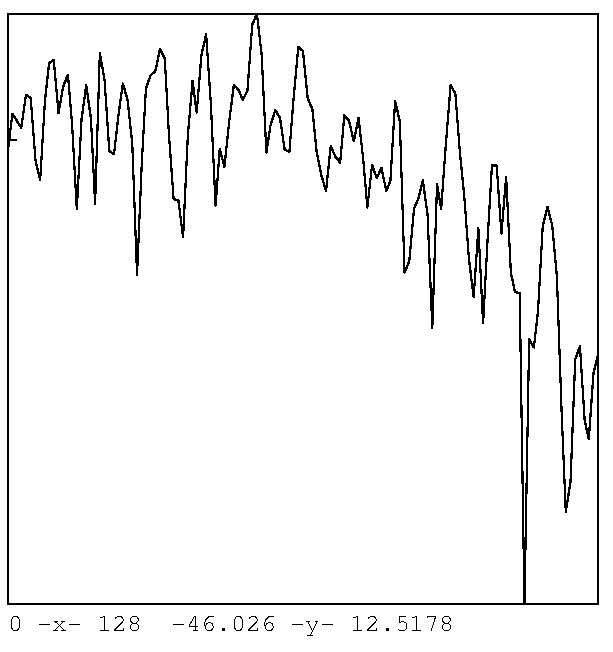
\includegraphics[width=6cm]{fig/train.pdf}
\end{center}
\end{qsection}

\begin{qsection}{SEE ALSO}
\hyperlink{impulse}{impulse},
\hyperlink{sin}{sin},
\hyperlink{step}{step},
\hyperlink{ramp}{ramp}
\end{qsection}


